% ---------------------------------------------------------------------------
% Section fragment: physical 2D simulation of the planned web (domain: sim)
% ---------------------------------------------------------------------------
\section{A Physical 2D Simulation of the Planned Web: Gravity, Wind and Moving Supports}
\label{sec:sim}

The web drawings produced by the planner's viewer (\texttt{visualization/index\_updated.html}) join plan nodes with
straight segments: a thread has no weight, no tension and no response to the environment. To show what the planned web
would look like as a physical object, we built a two-dimensional cable simulation of it. The simulation is a single
self-contained page, \texttt{simulation/orb\_web\_sim.html}. It takes the topology and construction order from the
same plan the viewer animates (\texttt{plan\_data\_updated.js}, 105 actions, 701.6\,cm of locomotory energy). It
adds gravity, so that every thread hangs in a catenary between its attachment points, and it turns the environmental
factors that the repository models abstractly (wind noise, anchor availability, moving supports, silk budget, damage)
into physical loads and boundary conditions. This section describes the model, the numerical scheme, a validation
against the analytic catenary and the results.

The simulation is an illustration layered on the planner's output. It is not a calibrated biomechanical model of silk
or of \emph{Araneus}, it does not feed back into planning, and none of its numbers supports any entry of the
project's claim ledger (\texttt{docs/research/CLAIMS.md}). The repository contains no silk-mechanics data, so every
material value below is illustrative and is labelled as such, both here and on the page.

\subsection{Model}
\label{sec:sim-model}

\paragraph{Geometry and topology from the plan.}
The web lies in the vertical plane of the rig in \texttt{spider\_web\_htn\_updated/config.yaml}: two 18\,cm sticks
16\,cm apart joined by a top and a bottom bar (the \texttt{walkable\_edges}), with the cross-bar at $y=9$\,cm drawn
but not touching the web. Plan nodes on this rectangle are fixed attachment points; all other nodes are free. We replay
the plan with the viewer's semantics. \texttt{lay\_thread}, \texttt{lay\_frame\_thread}, \texttt{lay\_radius} and
\texttt{build\_spiral\_segment} add a thread of the stated type. \texttt{insert\_radius} replaces the dragline between
an anchor and the hub by a proto-radius. Seven thread types are kept: bridge, dragline, proto-radius, frame, radius,
auxiliary spiral and capture spiral. Threads that meet share a node. Every thread is split wherever another thread's
endpoint lies on its chord: the hub, the radius--frame junctions and every waypoint at which a spiral segment
attaches to a radius. The finished web therefore has 66 threads, made of 2 bridges, 4 proto-radii, 4 frames,
8 radii, 20 auxiliary-spiral segments and 28 capture-spiral segments. It is meshed into 944 segments with 844 free
nodes at the default segment length of 0.5\,cm (at least two segments per span).

Two features of the plan have physical consequences. First, the plan places the proto-hub at $(8,12)$\,cm, which lies
on no earlier thread, so between the \texttt{anchor} action and \texttt{mark\_proto\_hub} the hub has no physical
support. The simulation holds it fixed as a construction scaffold until \texttt{mark\_proto\_hub} (step 24) and
releases it afterwards. Second, both spirals skip the bottom-right radius, because \texttt{spiral\_nodes} in the
configuration lists only seven of the eight radial anchors. That radius is therefore a single 13\,cm span carrying
almost no load.

\paragraph{Discretised tension-only cable.}
Each segment $s$ joins nodes $a$ and $b$ and has rest length $L_{0,s}$, axial stiffness $(EA)_s$ and linear density
$\mu_s$. Its elastic energy and tension are
\begin{equation}
  E_s = \frac{(EA)_s}{2L_{0,s}}\,\bigl(\ell_s - L_{0,s}\bigr)_+^2, \qquad
  T_s = (EA)_s\,\frac{(\ell_s - L_{0,s})_+}{L_{0,s}}, \qquad \ell_s = \lVert \mathbf{x}_b - \mathbf{x}_a \rVert ,
  \label{eq:sim-cable}
\end{equation}
where $(\cdot)_+ = \max(\cdot,0)$. A thread resists stretching but offers no resistance to compression, so a slack
segment simply carries no force. When a thread is laid, its rest length is the current chord times $(1+s_{\text{type}})$,
where $s_{\text{type}}$ is a per-type slack. A negative slack is a pretension. Masses are lumped at the nodes,
$m_i = \sum_{s\ni i} \tfrac12 X \mu_s L_{0,s}$. The factor $X$ is an explicit \emph{sag exaggeration}: it multiplies
the silk's mass and weight per unit length. With the illustrative values of Table~\ref{tab:sim-params}, a taut 16\,cm
radius at $X=1$ sags by 0.037\,cm, which is invisible at web scale, so the page and all figures use $X=2000$ unless
stated otherwise. The spider is a point mass (30\,mg, illustrative) that is not exaggerated. During each action it
moves along the thread being laid, or along the shortest path over built threads and rig edges for a \texttt{walk}
(the connectivity used by \texttt{operators.\_can\_reach}). Its weight is shared between the two nodes of the segment
it is on.

\begin{table}[htbp]
  \centering
  \caption{Parameters of the cable simulation and their sources. ``Illustrative'' means the value was chosen for
  plausible relative magnitudes and visibility; it does not come from a measurement. The capture spiral is given a
  20-fold lower stiffness than the radii to make it the most extensible thread.}
  \label{tab:sim-params}
  \footnotesize
  \begin{tabularx}{\linewidth}{@{}>{\raggedright\arraybackslash}X l l >{\raggedright\arraybackslash}p{0.27\linewidth}@{}}
    \toprule
    Quantity & Value & Unit & Source \\
    \midrule
    Linear density $\mu$: bridge, proto-radius, radius / dragline / frame & 0.10 / 0.08 / 0.15 & $\mu$g/cm & illustrative \\
    Linear density $\mu$: auxiliary / capture spiral & 0.05 / 0.20 & $\mu$g/cm & illustrative \\
    Axial stiffness $EA$: bridge, proto-radius, radius / dragline / frame & 60 / 40 / 100 & mN & illustrative \\
    Axial stiffness $EA$: auxiliary / capture spiral & 30 / 3 & mN & illustrative \\
    Slack $s$ (all types) & 0 & \% & illustrative \\
    Sag exaggeration $X$ & 2000 & -- & illustrative, explicit \\
    Gravity $g$ & 9.81 & m\,s$^{-2}$ & -- \\
    Normal drag coefficient $c_n$ ($c_t=c_n/2$) & $6\times10^{-5}$ & N\,s\,m$^{-2}$ & illustrative \\
    Gust strength \texttt{noise\_std} & 0.08 & -- & \texttt{config.yaml} (\texttt{stochastic.wind}) \\
    Gust time scale $\tau$ & 1 & s & illustrative \\
    Seed & 7107 & -- & \texttt{config.yaml} (\texttt{stochastic.seed}) \\
    Support amplitude $A$, frequency $f$ & 10, 0.05 (config: 0.049) & cm, Hz & \texttt{spider\_web\_mulder/\allowbreak config.yaml} \\
    Rig & $16\times18$ & cm & \texttt{spider\_web\_htn\_updated/\allowbreak config.yaml} \\
    Spider speed & 20 (repo: 1.0) & cm\,s$^{-1}$ & \texttt{spider\_web\_mulder/\allowbreak config.yaml}, sped up $20\times$ \\
    Spider mass & 30 & mg & illustrative \\
    Silk capacity & $\infty$ (perturbation: 2200) & cm & \texttt{perturbations.py} \\
    Segment length & 0.5 & cm & numerical \\
    \bottomrule
  \end{tabularx}
\end{table}

\paragraph{Catenary and parabola.}
A uniform cable of weight $w$ per unit length hanging between level supports a distance $L$ apart under horizontal
tension $H$ takes the shape
\begin{equation}
  y(x) = a\cosh\!\frac{x}{a} - a\cosh\!\frac{L}{2a}, \qquad a = \frac{H}{w}, \qquad
  d = a\Bigl(\cosh\frac{L}{2a}-1\Bigr) \approx \frac{wL^2}{8H},
  \label{eq:sim-catenary}
\end{equation}
with $x$ measured from mid-span. The small-sag limit is the parabola $y = -4d\,x'(L-x')/L^2$, with $x'$ measured from
one support. Our threads are extensible, so the exact reference for one span is the elastic catenary. In the
unstretched (Lagrangian) coordinate $p\in[0,L_0]$, with vertical support reaction $V = wL_0/2$,
\begin{equation}
  \begin{aligned}
  x(p) &= \frac{Hp}{EA} + \frac{H}{w}\Bigl[\operatorname{asinh}\frac{V}{H} - \operatorname{asinh}\frac{V-wp}{H}\Bigr],\\
  y(p) &= -\frac{Vp - wp^2/2}{EA} - \frac{\sqrt{H^2+V^2} - \sqrt{H^2+(V-wp)^2}}{w},
  \end{aligned}
  \label{eq:sim-elastic}
\end{equation}
where $H$ is fixed by the condition $x(L_0)=L$. For a span laid exactly taut ($s=0$), the sag comes only from elastic
stretch. Combining $d \approx wL^2/8H$ with $H \approx EA\cdot 8d^2/3L^2$ gives $(d/L)^3 \approx 3wL/(64\,EA)$, so
the sag scales as $(Xg)^{1/3}$.

\paragraph{Wind.}
The repository models wind as seeded multiplicative Gaussian noise on movement cost (\texttt{stochastic.wind\_noise\_factor}:
a factor $1+\mathcal N(0,\texttt{noise\_std}^2)$ floored at 0.1). In the simulation, wind is a physical load. The
in-plane air velocity is $\mathbf w(t) = U\,\max\{1+\sigma\xi(t),\,0.1\}\,\hat{\mathbf e}_\theta$, where $\sigma$ is
\texttt{noise\_std}, $\xi$ is a seeded unit-variance Ornstein--Uhlenbeck process with time scale $\tau$, and
$\hat{\mathbf e}_\theta$ is the wind direction. The drag per unit length on a thread with tangent $\mathbf t$ is linear,
as appropriate for micrometre fibres at low Reynolds number:
\begin{equation}
  \mathbf f = c_n\,(\mathbf I - \mathbf t\mathbf t^{\mathsf T})(\mathbf w - \mathbf v) + c_t\,\mathbf t\mathbf t^{\mathsf T}(\mathbf w - \mathbf v),
  \label{eq:sim-drag}
\end{equation}
which also provides physical damping. Only the in-plane component of wind is represented. In reality the wind load on
an orb web is mostly normal to its plane, so the 2D model shows how the web bellies within its plane and not how it
billows out of it. Because only the weight is exaggerated, the ratio of wind load to weight here is $X$ times smaller
than it would be for silk of the stated density.

\paragraph{Moving supports, anchors, silk budget, damage.}
Support motion uses the affine shear of \texttt{spider\_web\_mulder/model.py},
$x \mapsto x + (1 - y/H_{\text{rig}})\,A\sin(2\pi f t+\phi)$ with $H_{\text{rig}}=18$\,cm, applied to the fixed rig
nodes: the top bar is fixed and the bottom bar moves. Anchor availability reproduces
\texttt{stochastic.select\_available\_anchors} exactly. The page contains a Python-compatible MT19937 generator, so
for a given seed and removal probability it removes the same anchors as Python \texttt{random.Random(seed)} drawing
over the sorted removable anchors. We checked this against Python for six seeds. A thread is not built if it ends on a
removed anchor, or on a spiral waypoint that lies on that anchor's radius. Unlike the planner, the page does not
replan. The silk budget follows \texttt{operators.\_has\_capacity}: construction stops at the first action whose
cumulative plan distance exceeds the capacity. Structural failure after construction (cf.\ \texttt{perturbations.py})
is modelled by releasing an anchor, so that its threads fall under load.

\subsection{Numerical scheme}
\label{sec:sim-numerics}

Each time step is a backward-Euler step written as the minimisation of an incremental potential. With the positions
$\mathbf x^n$ and velocities $\mathbf v^n$ of the free nodes, the predicted position $\hat{\mathbf x} = \mathbf x^n + h\mathbf v^n$
and the drag tensor $\mathbf D$ assembled from Eq.~\eqref{eq:sim-drag} at $\mathbf x^n$, the new positions solve
\begin{equation}
  \mathbf x^{n+1} = \arg\min_{\mathbf x}\;
  \tfrac{1}{2h^2}\lVert\mathbf x-\hat{\mathbf x}\rVert^2_{\mathbf M}
  + \tfrac{1}{2h}(\mathbf x-\mathbf x^n)^{\mathsf T}(\mathbf D + c\mathbf M)(\mathbf x-\mathbf x^n)
  - \mathbf F^{\mathsf T}(\mathbf x-\mathbf x^n) + \sum_s E_s(\mathbf x),
  \label{eq:sim-ip}
\end{equation}
where $\mathbf F$ collects weight, the drag force $\mathbf D\mathbf w$ and the spider's load, and $c=0.5\,\text{s}^{-1}$
is a small numerical damping. Each $E_s$ is convex (a non-decreasing convex function of the convex $\ell_s$), so the
objective is strictly convex. We minimise it by Newton's method with the exact tension-only Hessian
$k_s[\mathbf n\mathbf n^{\mathsf T} + (1-L_{0,s}/\ell_s)(\mathbf I-\mathbf n\mathbf n^{\mathsf T})]$ for taut segments,
with $k_s=(EA)_s/L_{0,s}$, and an Armijo line search on the objective. This combination cannot diverge, and the step
is clamped to $h=1/120$\,s (two sub-steps per 1/60\,s frame). The linear systems are solved exactly by $2\times2$-block
Gaussian elimination in minimum-degree order: thread chains are eliminated first, at no cost in fill. The
\emph{settle} operation computes static equilibrium by the same Newton iteration with the inertia term replaced by an
adaptive Levenberg--Marquardt proximal term. It stops when the largest unbalanced nodal force is below $10^{-6}$ of the
largest applied nodal force (below $10^{-7}$ for the validation span). Starting from the planned straight lines, the
finished web settles in about 70 Newton iterations (about 40\,ms in the browser). At rest the kinetic energy decays to
about $10^{-36}$\,J and stays there, so the web does not creep or jitter. For slack spans the solver starts from a
parabola of the correct arc length; this affects speed only, because the minimiser is unique for $g>0$.

We use two ways of building a web. A \emph{history-free} build lays every thread alive after step $k$ on the planned
straight lines at once and then settles; this is the ``finished web'' of the page. A \emph{quasi-static sequential}
build executes the 105 actions in order and settles after each one, so that every new thread is laid between the
current, already sagged positions of its attachment points. All 105 sequential settles converged (worst relative
residual $9.4\times10^{-7}$). Live playback integrates Eq.~\eqref{eq:sim-ip} in real time while the spider walks.
Newton iterations per time step are capped at 60. In a full playback at the default spider speed no step reached the
cap. The largest tension seen during playback, 1.8\,mN against 1.44\,mN in the final settled state, is the dynamic
effect of the walking spider: without it, the playback peak (0.557\,mN) equals the static value. Zero-slack threads put many segments exactly at the slack/taut kink of Eq.~\eqref{eq:sim-cable}, where Newton can need tens of
iterations; a tighter cap leaves steps unconverged and produces spurious tension spikes.

\subsection{Validation against the catenary}
\label{sec:sim-validation}

The page's second panel simulates one thread between two level supports with the same \texttt{World} solver. It
draws the result over Eq.~\eqref{eq:sim-elastic}, the rigid catenary of Eq.~\eqref{eq:sim-catenary} with the same $H$
and $w$, and the parabola (Fig.~\ref{fig:sim-validation}). For a 16\,cm span of radius material at $X=2000$:
\begin{itemize}
  \item With 40 segments and no slack, the largest distance between a simulated node and the exact elastic catenary is
        0.97\,$\mu$m, or 0.02\% of the 0.465\,cm sag. The simulated horizontal tension, 0.13476\,mN, is within
        0.02\% of the exact $H=0.13479$\,mN.
  \item The error falls as $N^{-2}$ from $N=4$ to $N=256$ at 0, 1 and 5\% slack
        (Fig.~\ref{fig:sim-validation}c). This is the expected behaviour of a lumped-mass discretisation, so the
        remaining error is discretisation error and not a solver bias.
  \item At $N=40$ the error grows with sag, to 15\,$\mu$m at 20\% slack (4.7\,cm sag). Even there it is more than two
        orders of magnitude smaller than the error of the parabolic approximation, which is 250\,$\mu$m at 3\% slack
        and 4.2\,mm at 20\% slack.
\end{itemize}
The simulated sag is therefore physically right for the model of Eq.~\eqref{eq:sim-cable}: it is computed, not drawn
on. The web uses 0.5\,cm segments, so a 16\,cm span has 32 segments, which by Fig.~\ref{fig:sim-validation}c puts the
discretisation error in the micrometre range. For orientation, the same span at $X=1$ sags by 0.037\,cm.

\begin{figure}[htbp]
  \centering
  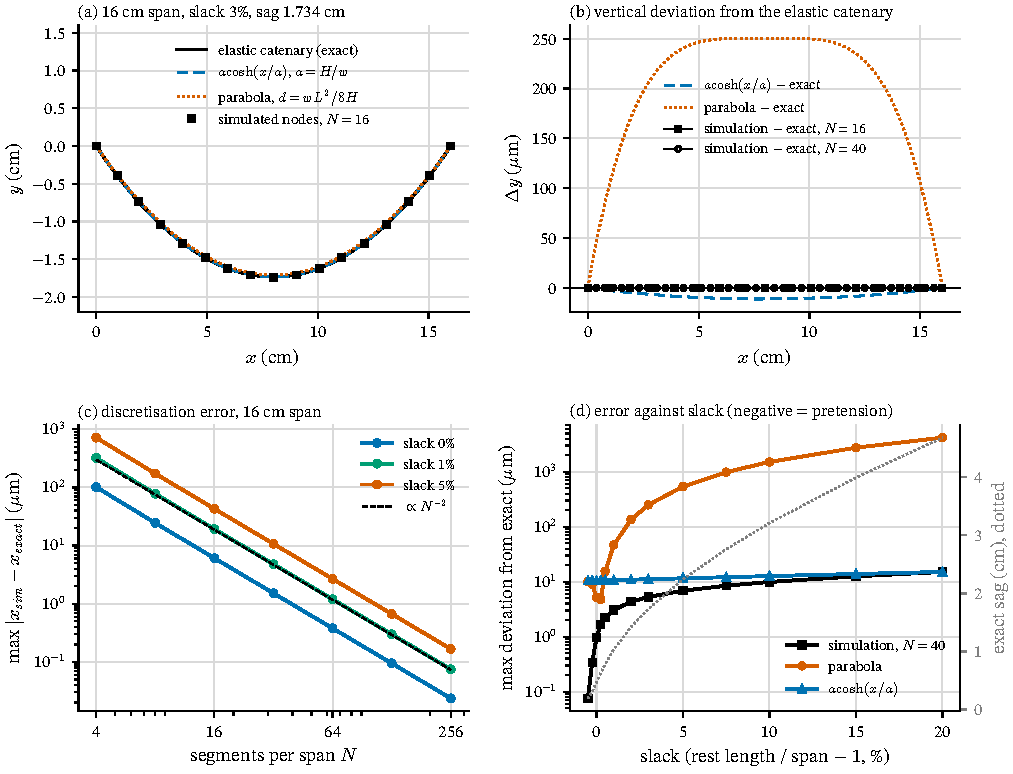
\includegraphics[width=\linewidth]{figures/sim/sim_validation}
  \caption{Validation of the cable solver on one 16\,cm span ($\mu=0.10\,\mu$g/cm, $EA=60$\,mN, $X=2000$, level
  supports). (a)~Shape at 3\% slack with $N=16$ segments against the elastic catenary (Eq.~\ref{eq:sim-elastic}),
  the rigid catenary $a\cosh(x/a)$ with the same $H$ and $w$, and the parabola $d=wL^2/8H$. (b)~Vertical deviation of
  each curve from the elastic catenary. (c)~Largest node error against $N$ for 0, 1 and 5\% slack; dashed line
  $\propto N^{-2}$. (d)~Largest deviation from the exact curve against slack at $N=40$ (negative slack = pretension);
  the dotted line is the exact sag (right axis). $n=21$ runs in (c) and 13 in (d); the runs are deterministic, so
  there are no error bars. Data: our runs of \texttt{simulation/orb\_web\_sim.html} (\texttt{report/scripts/sim/evals/validation.js}).}
  \label{fig:sim-validation}
\end{figure}

\subsection{Results}
\label{sec:sim-results}

\paragraph{Gravity and wind.}
With $g=0$ the settled web coincides with the straight-line plan to machine precision (Fig.~\ref{fig:sim-web}a).
With gravity, every span hangs in a smooth downward curve (Fig.~\ref{fig:sim-web}b). No span between junctions rises
above its chord. In the intermediate states where they carry nothing else, the vertical radius (after step 52) stays
straight to $4\times10^{-7}$\,cm, and the bottom frame (after step 32) sags by 0.449\,cm, symmetrically to
round-off. Kinks occur only at junctions, where other threads pull, as in a real net.
With the 30\,mg spider on the hub, the hub drops by 0.067\,cm to $y=11.933$\,cm. The largest thread sag, 0.96\,cm, is
on the longest capture-spiral span (8.9\,cm chord), and the largest tension, 0.94\,mN, is on a radius. Without the
spider the largest tension is 0.57\,mN. The capture spiral is the most compliant thread type, at the bottom of the
tension distribution (median per-thread maximum 0.028\,mN against 0.090\,mN for the radii; Fig.~\ref{fig:sim-tension}).

A steady 4\,m/s wind in the $+x$ direction bows the web downwind and raises the maximum sag to 1.15\,cm
(Fig.~\ref{fig:sim-web}c). The node displacement relative to still air grows steeply between 1 and 2\,m/s, from 0.27
to 0.82\,cm, and more slowly after that (1.03\,cm at 8\,m/s; Fig.~\ref{fig:sim-sweeps}a). The thread that moves most
in that range is the bottom-right radius. Because no spiral attaches to it, it carries only about 0.05\,mN and swings
sideways under a small load. Wind directed downwards instead mainly raises the tension, from 0.57 to 1.27\,mN at
8\,m/s.

\begin{figure}[htbp]
  \centering
  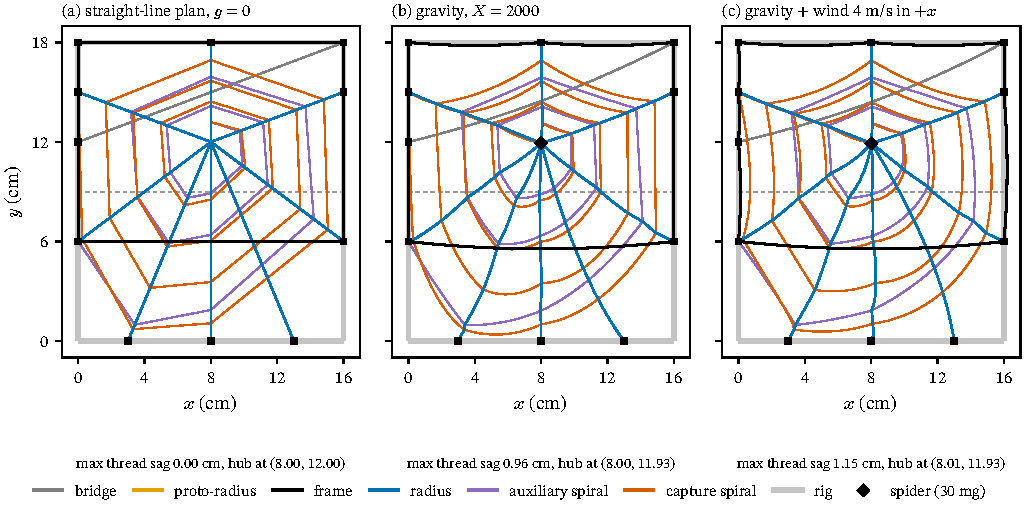
\includegraphics[width=\linewidth]{figures/sim/sim_web_states}
  \caption{The finished planned web at the same scale. (a)~$g=0$: identical to the straight-line plan.
  (b)~Static equilibrium under gravity with sag exaggeration $X=2000$. (c)~The same with a steady 4\,m/s in-plane wind
  towards $+x$. Spider (30\,mg) at the hub; material values illustrative (Table~\ref{tab:sim-params}). Each panel is
  one deterministic run with 66 threads. Data: our runs of \texttt{simulation/orb\_web\_sim.html}, which embeds the
  plan of \texttt{visualization/plan\_data\_updated.js} (\texttt{report/scripts/sim/evals/web\_states.js}).}
  \label{fig:sim-web}
\end{figure}

\paragraph{Construction under gravity.}
Figure~\ref{fig:sim-phases} shows the quasi-static sequential build at the end of each macro phase. Physically
interesting intermediate states appear that the straight-line viewer cannot show. After proto-hub establishment the
two upper proto-radii, which carry the hub, are nearly straight, while the two lower ones hang in visible catenaries. The auxiliary-spiral segments near the bottom-left anchor hang in deep loops. Construction history matters.
Compared with the history-free build, the sequentially built web has its hub 0.27\,cm lower ($y=11.66$\,cm), a
larger maximum tension (1.40 against 0.94\,mN), and node positions that differ by up to 1.38\,cm. The reason is that
each thread inherits the sag of the web on which it was laid.

\begin{figure}[htbp]
  \centering
  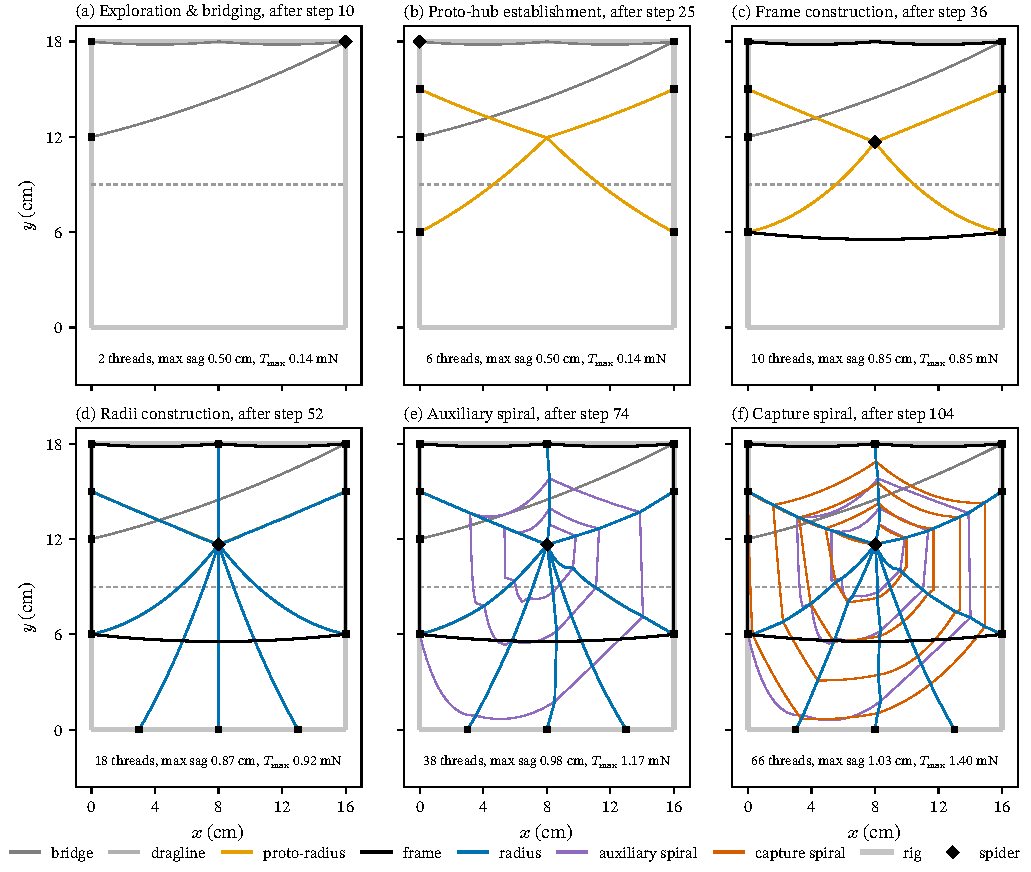
\includegraphics[width=\linewidth]{figures/sim/sim_construction_phases}
  \caption{Quasi-static sequential construction under gravity ($X=2000$): the web after the last action of each macro
  phase of the HTN plan (steps 10, 25, 36, 52, 74 and 104 of 105; step 105, \texttt{mark\_web\_complete}, adds no
  thread). Each new thread is laid between the current positions of its attachment points, and the web is settled
  after every action. One deterministic run with 105 settles, all converged. Data: our run of
  \texttt{simulation/orb\_web\_sim.html} on the plan in \texttt{visualization/plan\_data\_updated.js}
  (\texttt{report/scripts/sim/evals/phases.js}).}
  \label{fig:sim-phases}
\end{figure}

\paragraph{Sag and tension as functions of the factors.}
Slack and pretension behave as expected (Fig.~\ref{fig:sim-sweeps}b). Going from 1\% pretension to 4\% slack on
every thread raises the bottom-frame sag from 0.10 to 2.0\,cm and lowers the maximum tension from 1.59 to 0.46\,mN.
Varying $X$ and varying $g$ give the same sag for the same product $Xg$ (Fig.~\ref{fig:sim-sweeps}c), as the statics
require. For the taut bottom frame the sag follows the $(Xg)^{1/3}$ law derived above over five decades. The maximum
sag over the whole web levels off at low weight (0.20\,cm at $X=1$). With no pretension the unloaded net is a
mechanism: a tiny load moves the junctions slightly, which shortens some chords and leaves those spans geometrically
slack. Real webs are pretensioned. The page can represent this with negative slack, but it has no data from which to
set the value.

\begin{figure}[htbp]
  \centering
  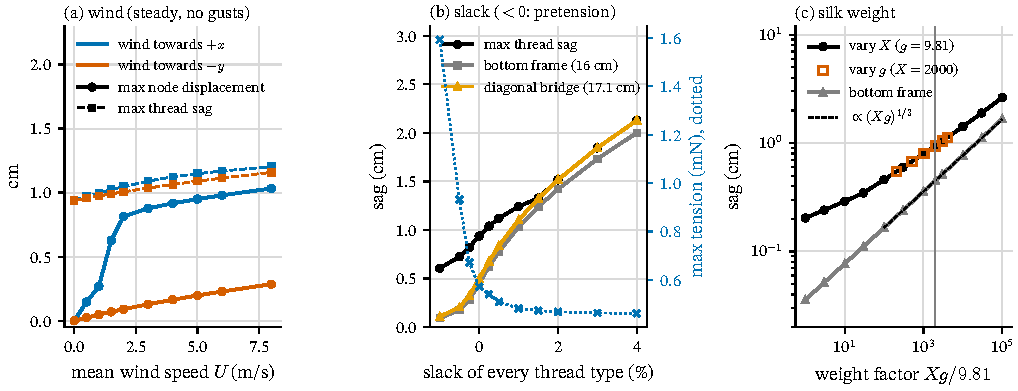
\includegraphics[width=\linewidth]{figures/sim/sim_sag_sweeps}
  \caption{Static response of the finished web (spider load off). (a)~Largest node displacement relative to still
  air (solid) and largest thread sag (dashed) against steady wind speed, for wind towards $+x$ and towards $-y$.
  (b)~Sag against the slack applied to every thread type (negative = pretension), with the largest tension (dotted,
  right axis). (c)~Sag against the weight factor $Xg/9.81$, from a sweep of $X$ at $g=9.81$ and a sweep of $g$ at
  $X=2000$; dashed line $\propto(Xg)^{1/3}$. $n=20$, 11, 12 and 7 deterministic runs. Data: our runs of
  \texttt{simulation/orb\_web\_sim.html} (\texttt{report/scripts/sim/evals/sweeps.js}).}
  \label{fig:sim-sweeps}
\end{figure}

\begin{figure}[htbp]
  \centering
  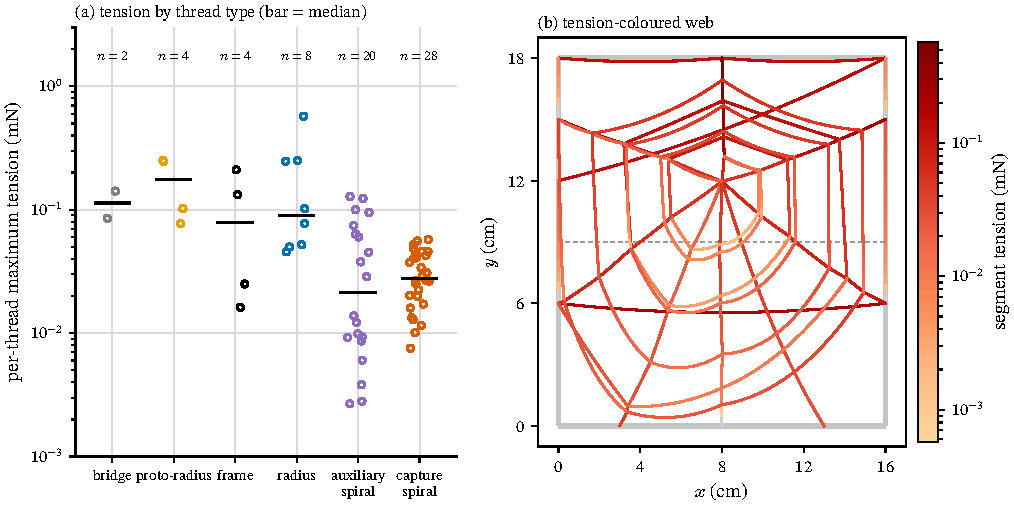
\includegraphics[width=\linewidth]{figures/sim/sim_tension}
  \caption{Tension in the finished web under gravity ($X=2000$, spider load off). (a)~Maximum tension of each thread
  by type; the bar is the median, and $n$ (threads per type) is printed above each column. (b)~Segment tension on a
  logarithmic colour scale (944 segments; light grey would mark segments below $10^{-3}$ of the maximum). Data: our
  run of \texttt{simulation/orb\_web\_sim.html} (\texttt{report/scripts/sim/evals/web\_states.js}).}
  \label{fig:sim-tension}
\end{figure}

\paragraph{Moving supports.}
Under the Mulder package's 10\,cm, 0.05\,Hz shear the rig deforms into a parallelogram and the web follows it
(Fig.~\ref{fig:sim-supports}). The hub swings by $\pm3.7$\,cm, the maximum tension rises from 0.94\,mN at the neutral
phase to 20.9\,mN at full displacement (always on a radius), and the peak strain reaches 35\%. Real silk might fail at
such strains, but the repository has no breaking-strain data, so the simulation does not model failure. At 5\,cm the
peak tension is 8.1\,mN (strain 13.5\%). Doubling the frequency to 0.1\,Hz leaves the tension history unchanged, and
the kinetic energy never exceeds $10^{-7}$\,J. At the support frequencies of Mulder et al.~\cite{mulder2021dynamic}, as
modelled in the repository, the web's response is therefore quasi-static: the loads come from the change of support
geometry and not from inertia. Because the motion is an affine shear, threads whose rest length was set at the
neutral phase are alternately stretched and slackened. This is visible in the slack, zig-zag radii at the extreme
phases.

\begin{figure}[htbp]
  \centering
  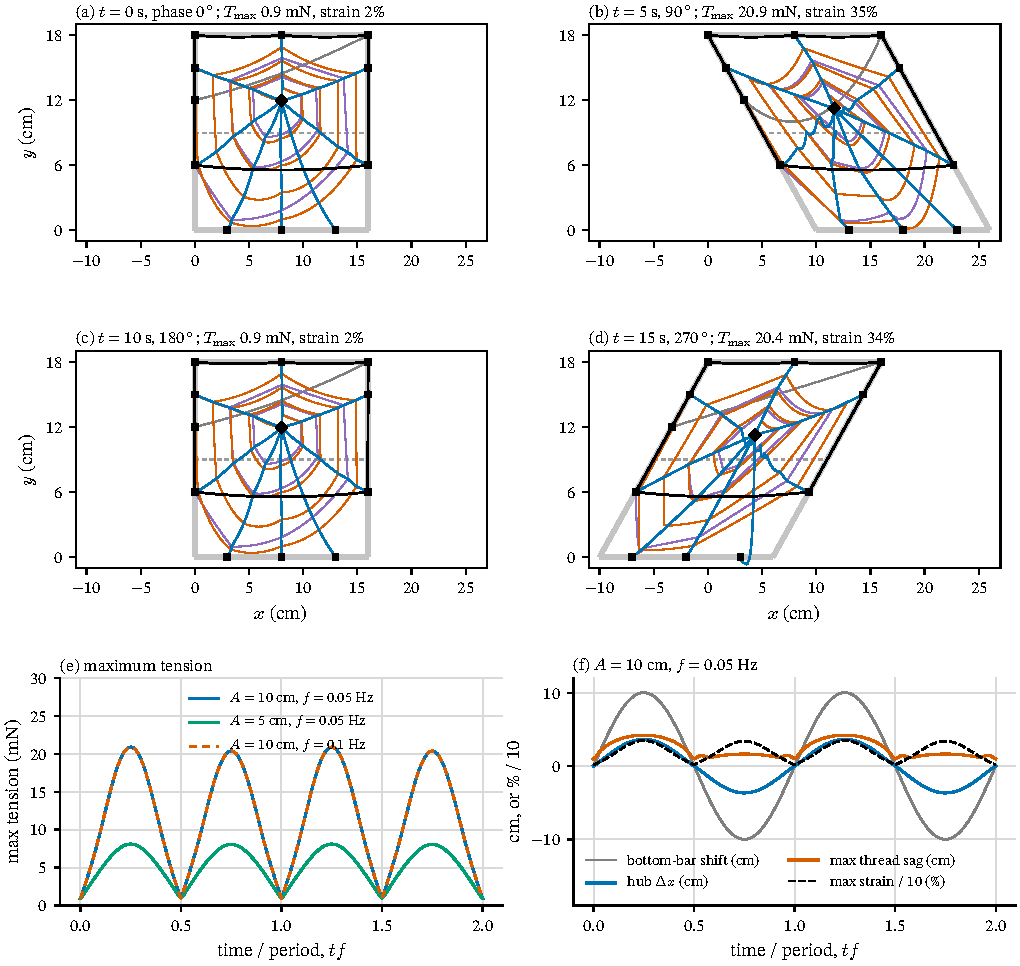
\includegraphics[width=\linewidth]{figures/sim/sim_moving_supports}
  \caption{Moving supports: the affine shear $x\mapsto x+(1-y/18\,\text{cm})A\sin(2\pi ft)$ of
  \texttt{spider\_web\_mulder/\allowbreak model.py} applied to the rig, starting from the settled finished web. (a--d)~$A=10$\,cm,
  $f=0.05$\,Hz at phases 0, 90, 180 and 270$^\circ$. (e)~Maximum tension over two periods for three conditions; the
  0.1\,Hz curve (dashed) coincides with the 0.05\,Hz curve. (f)~Bottom-bar shift, hub displacement, maximum thread sag
  and maximum strain for $A=10$\,cm, $f=0.05$\,Hz. Three deterministic runs, 161 samples each. Data: our runs of
  \texttt{simulation/orb\_web\_sim.html} (\texttt{report/scripts/sim/evals/supports.js}).}
  \label{fig:sim-supports}
\end{figure}

\paragraph{Anchor availability and damage.}
Figure~\ref{fig:sim-anchors} uses the same anchor draws as the planner's sensitivity runs. For a fixed seed the
removed sets are nested as $p$ grows. Removing the top-centre and right-upper anchors (seed 7107, $p=0.35$) leaves the
hub supported mainly from the left, and it falls from $(8.0,11.9)$ to $(6.4,9.2)$\,cm. The webs shown are the planned
web minus the threads that cannot be built. They are not the webs the planner would produce, because the planner
replans around missing anchors and the page does not. Releasing one anchor after construction moves the hub by less than
0.01\,cm. How far the rest of the web moves depends on what else holds the freed node (Fig.~\ref{fig:sim-detach}).
The end of the bottom-left radius is held by the spiral junctions above it, and no node moves by more than 0.92\,cm.
The freed right-lower anchor is pulled into a deep loop by the bottom frame, and nodes move by up to 3.8\,cm.

\begin{figure}[htbp]
  \centering
  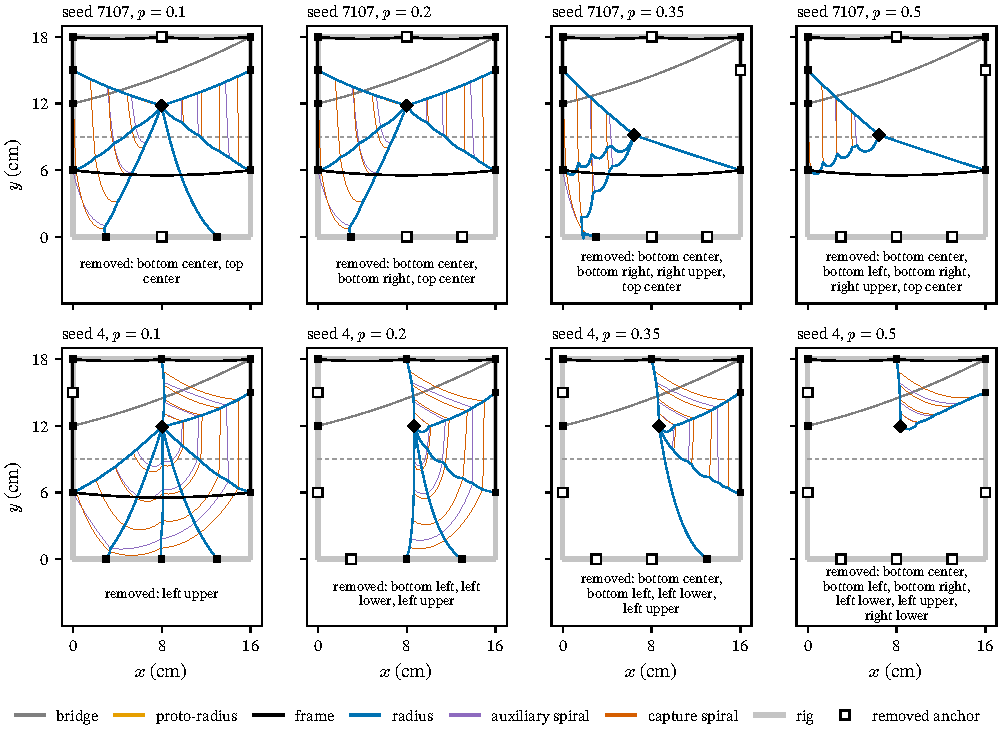
\includegraphics[width=\linewidth]{figures/sim/sim_anchor_removal}
  \caption{Seeded anchor removal at increasing probability $p$ for seed 7107 (the configuration seed) and seed 4.
  Anchors are drawn exactly as in \texttt{stochastic.select\_available\_anchors}; hollow squares mark removed anchors.
  Threads ending on a removed anchor, or on a spiral waypoint of its radius, are not built, and there is no replanning.
  Static equilibria, $X=2000$; eight deterministic runs. Data: our runs of \texttt{simulation/orb\_web\_sim.html}
  (\texttt{report/scripts/sim/evals/anchors.js}); removable anchors and seed from
  \texttt{spider\_web\_htn\_updated/config.yaml}.}
  \label{fig:sim-anchors}
\end{figure}

\begin{figure}[htbp]
  \centering
  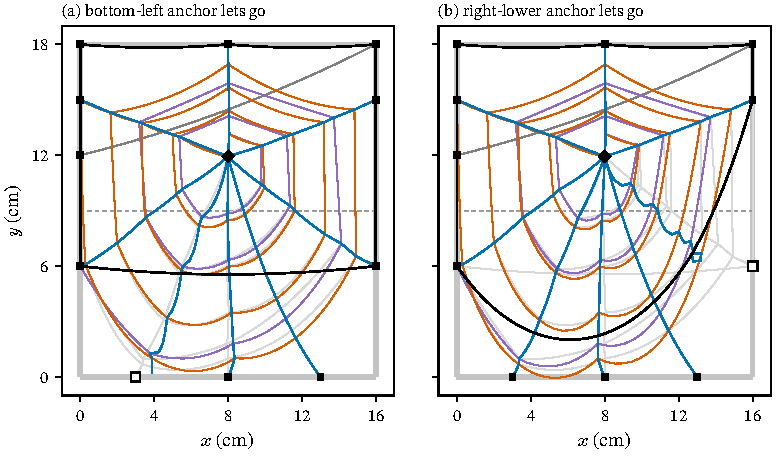
\includegraphics[width=0.78\linewidth]{figures/sim/sim_detach}
  \caption{Structural failure after construction (cf.\ \texttt{perturbations.py}): (a)~the bottom-left or
  (b)~the right-lower anchor lets go, and the web settles to a new equilibrium; the original web is shown in light
  grey. Two deterministic runs. Data: our runs of \texttt{simulation/orb\_web\_sim.html}
  (\texttt{report/scripts/sim/evals/anchors.js}).}
  \label{fig:sim-detach}
\end{figure}

\subsection{The simulation page}
\label{sec:sim-page}

The page (Fig.~\ref{fig:sim-page}) is deliberately plain: a figure with axis ticks in centimetres, a dense parameter
table that names the repository source of each control, and numerical readouts. The readouts are silk length by type,
maximum thread and span sag and where they occur, maximum tension and strain, hub position, kinetic energy, wind speed
and the plan's locomotory energy so far, with live traces. It supports play, pause, single-step and scrubbing through
the plan, a ``finished web'' mode, tension colouring and an overlay of the straight-line plan. Every setting is also a
URL parameter, for example
\texttt{?mode=final\&\allowbreak g=9.81\&\allowbreak exag=2000\&\allowbreak wind=2\&\allowbreak dir=0\&\allowbreak gust=0.3\&\allowbreak seed=7\&\allowbreak drop=0.2\&\allowbreak amp=10\&\allowbreak freq=0.05\&\allowbreak panel=validate\&\allowbreak ui=0}.
A global \texttt{window.simAPI} offers \texttt{set}, \texttt{buildTo}, \texttt{buildQuasiStatic}, \texttt{settle},
\texttt{advance}, \texttt{metrics}, \texttt{threads}, \texttt{validate}, \texttt{detach} and \texttt{render}. All runs
are deterministic for a given seed. Every number and figure in this section was produced through \texttt{simAPI}; the
scripts are in \texttt{report/scripts/sim/}.

\begin{figure}[htbp]
  \centering
  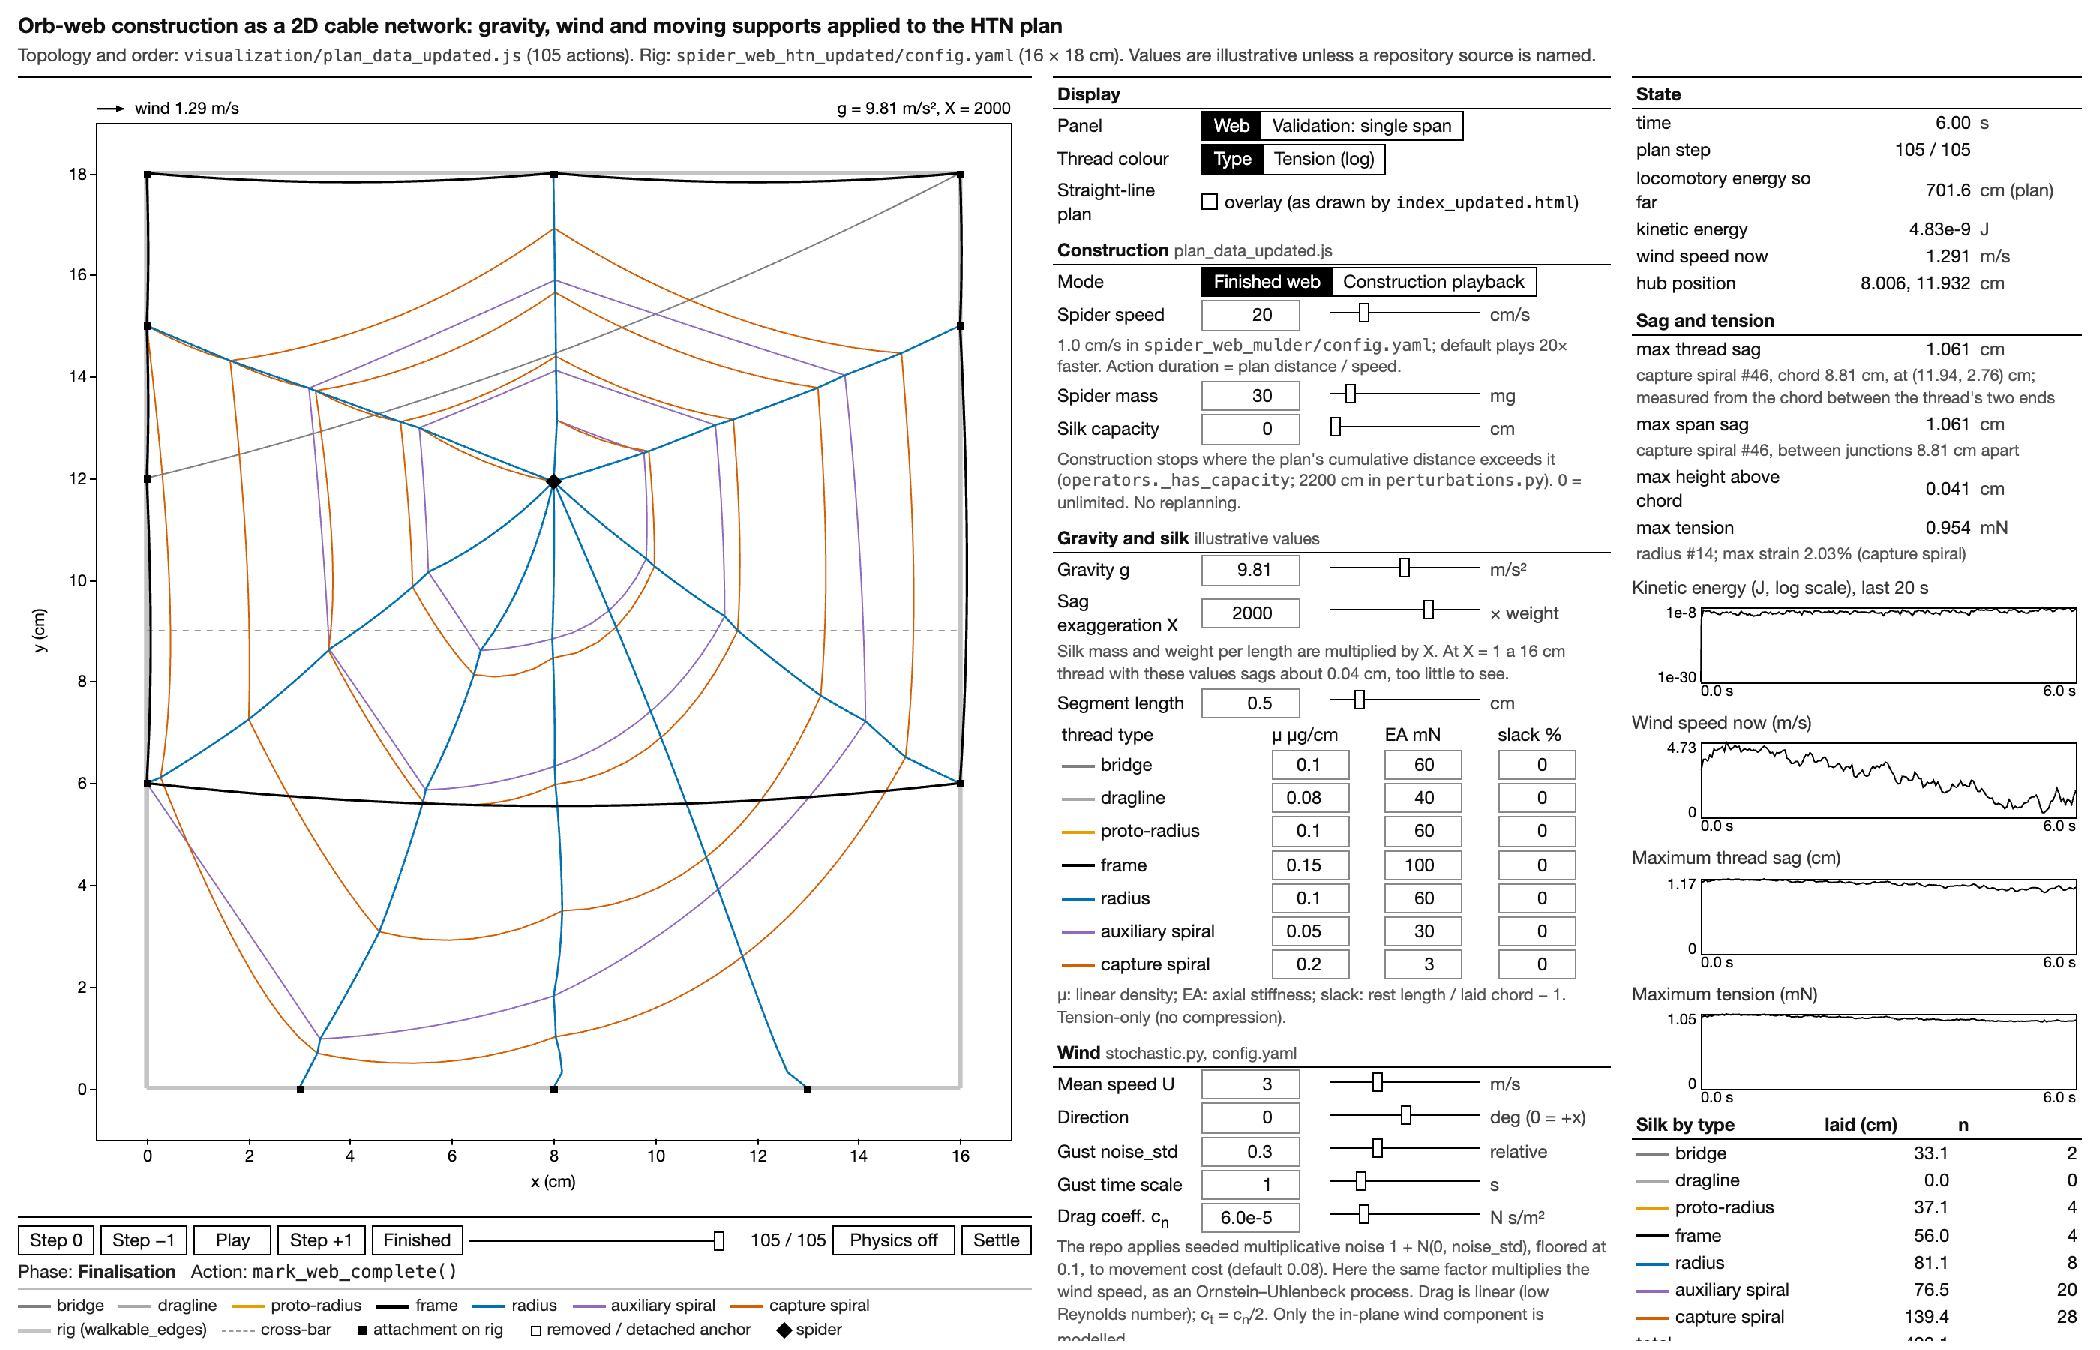
\includegraphics[width=\linewidth]{figures/sim/sim_page}
  \caption{The simulation page (\texttt{simulation/orb\_web\_sim.html}) at $1400\times900$ px, showing the finished web
  after 6\,s of gusty wind ($U=3$\,m/s, \texttt{noise\_std} $=0.3$, seed 7) with the parameter table, readouts and
  live traces. One capture.}
  \label{fig:sim-page}
\end{figure}

\subsection{Scope and limitations}
\label{sec:sim-scope}

The simulation is a physical illustration of the planner's output, with exaggerated and otherwise illustrative
parameters. The repository holds no measured silk density, stiffness, pretension, breaking strain, drag coefficient or
spider mass, so the absolute sags and tensions reported here carry no biological meaning. What can be stated is the
following: the solver reproduces the analytic catenary to within 0.02\% of the sag; the trends with slack, weight,
wind and support motion are those of a tension-only cable net; and the planned geometry has specific mechanical
features, namely an unsupported proto-hub before \texttt{mark\_proto\_hub}, an unloaded bottom-right radius, and slack
lower proto-radii during construction. The model is two-dimensional, so out-of-plane wind (the dominant real load) and
contact with the cross-bar are not represented. Threads do not break and do not interact where they cross without a
plan junction. The auxiliary spiral, which real spiders remove while laying the capture spiral, is kept because the
plan keeps it. Spiral attachment and anchor removal follow the embedded plan without replanning. The simulation feeds
no claim in \texttt{docs/research/CLAIMS.md}.
